

\documentclass{beamer}
\usepackage[utf8]{inputenc} 
\usepackage[T1]{fontenc}
\usepackage[spanish]{babel}
\usepackage{color}



\title{La comercializacion actual de productos alimenticios y bebidas en el municipio Centro Habana}
\date{Universidad de La Habana\\Facultad de Matematica y Computación}
\author{Vicente Cao Tarrero}
\centering

\includegraphics[scale=0.3]{matcom.png}
\usetheme{bars}
\usecolortheme{default}
\setbeamercovered{transparent}


\begin{document}
\begin{frame}
\titlepage{}
\end{frame}

\begin{frame}{Cerveza}
    El grafico muestra la diferencia entre el precio y el contenido en ml.
    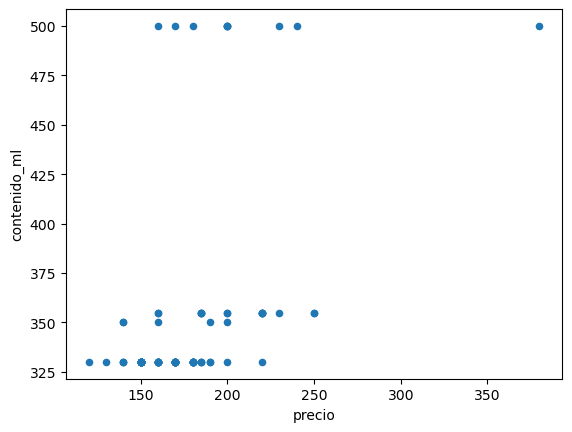
\includegraphics[scale=0.5]{Cerv_tipo_de_envace_precio.png}
    \end{frame}

\begin{frame}{Cerveza}
    Se representa en el grafico el color de envace que mas predomina.
    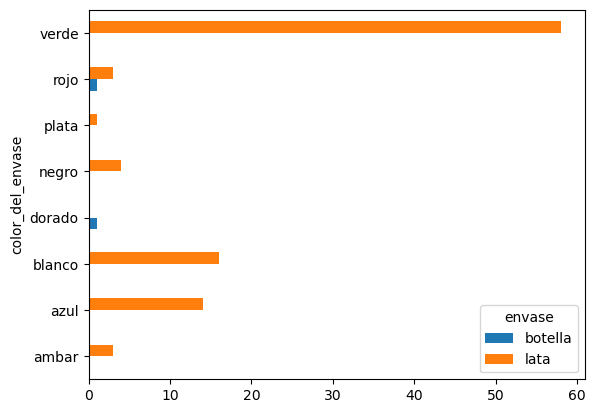
\includegraphics[scale=0.5]{Cerv_tipo_de_envace.png}
    \end{frame}

\begin{frame}{Cerveza}
    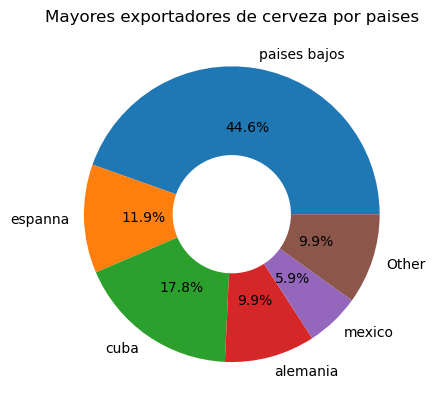
\includegraphics[scale=0.5]{Cerv_mayor_exportador.png}
    \end{frame}

\begin{frame}{Cerveza}
    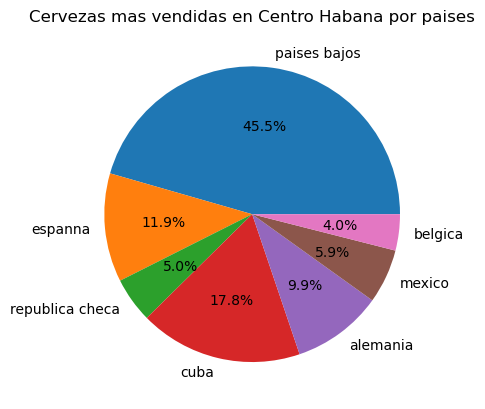
\includegraphics[scale=0.5]{Cerv_mas_vendida_por_pais.png}
    \end{frame}

\begin{frame}{Cerveza} 
    Cerveza mas vendida en Centro Habana.
    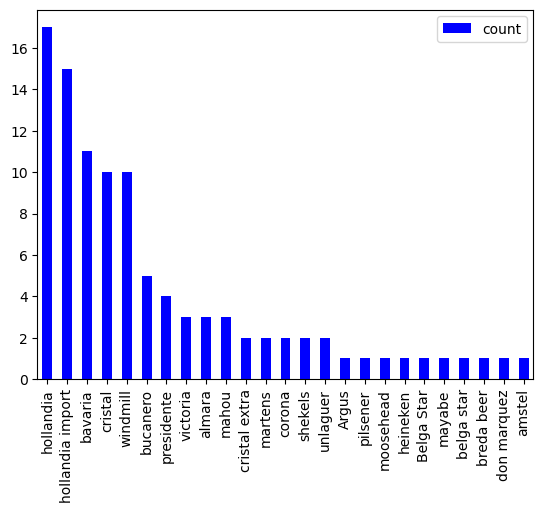
\includegraphics[scale=0.5]{Cerv_mas_vendida.png}
    \end{frame}

\begin{frame}{Cebolla}
    Formas de comercializacion de la cebolla.
    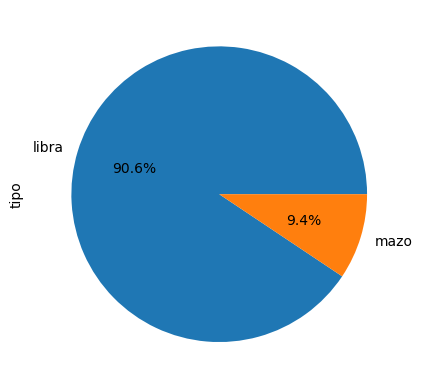
\includegraphics[scale=0.5]{Ceb_tipos_de_ventas.png}
    \end{frame}

 \begin{frame}{Cebolla}
    Variedad de cebolla mas vendida segun la coloracion
    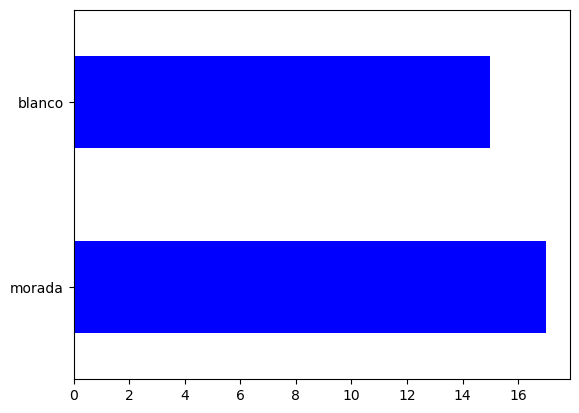
\includegraphics[scale=0.5]{Ceb_mas_vendida.png}
    \end{frame}   

    
\end{document}